We shall consider an example of a real-life optimal design problem, and explore a range of solutions provided by the compound criteria constructed in previous sections.
A company specialising in food supplements production for small animals were to conduct an experiment to figure out whether a slight decrease in the recommended dosages of three particular products taken together would make a significant impact on the resulting ``performance'', which is expressed in terms of some continuous response. The dosage range of interest for each supplement (experimental factor) is from $90\%$ to $100\%$ of the standard recommendation; it is desired that there would be $3$ levels (i.e. taking the values of $90\%$, $95\%$ and $100\%$). Carrying out the experiment with more than $3$ levels was more complicated: measuring, for example, $92.5\%$ of the recommended dosage was quite tricky. 

The treatments were to be applied to $n = 36$ cages of animals (experimental units), which would be allocated in $b=2$ equal sized blocks. The fullest response surface model, therefore, would contain all linear, quadratic and interaction terms: the primary model contains $p=9$ terms. As it was suspected that increasing dosages beyond certain values might not be of an impact, that would be translated in a non-quadratic curvature of the fitted function -- meaning that a presence of higher order terms would provide a better fit for the data, and it was desirable to accommodate for that possibility at the design stage. In the extended model We accounted for $q=10$ potential terms ((linear-by-linear-by-linear, quadratic-by-linear and cubic) in the extended model, with the notations the same as before:
\begin{equation*}
\bm{Y}=\bm{Z\beta}_{B}+\bm{X}_{p}\bm{\beta}_{p}+\bm{X}_{q}\bm{\beta}_{q}+\bm{\varepsilon},
\end{equation*}

The design search was performed among a larger $5$-level candidate set of points, but due to the form of the $2$nd order polynomial primary model and the criteria used, the resulting designs were $3$-level ones. The experimenters also wished to have at least two centre points in each block to ensure representation of the conditions thought a priori most likely to be best (with dosages of $95\%$ for each supplement), i.e. $4$ runs in total were fixed beforehand; this constraint was built directly into the search procedure; we also obtained designs without this restriction and evaluated the efficiency losses.

The experimenters preferred using the determinant-based criterion  as the primary inferential interest is on the overall input of the model terms; we searched for exact optimal designs with respect to the compound MSE(DP)-criteria for blocked experiments (\ref{eq::MSE_B_det}). For each combination of weights we will consider two cases: $\tau^2=1$ and $\tau^2=1/q$; as for the number of Monte Carlo samples used to estimate the third criterion component, for$\tau^2=1$ we set $N=500$, and for $\tau^2=1/q$ we set $N=1000$ in order to have a sufficiently small relative estimation error ([cite the thesis?]). The search for each design was performed with $50$ random starts.
We considered three sets of weights: (1) with the weight being equally distributed between the components, (2) a bit more weight ($0.4$) put on the DP-component, with the rest allocated to the lack-of-fit component, and (3) with half of the weight on the $MSE(D)$-component with the rest of it distributed evenly among the others. 

%%% MSE(D)-optimal designs, WITHOUT centre points: DP, LoF(DP) and MSE(D)
Table \ref{tab::MSE(D)_caseCP} contains the summaries of the optimal designs; the two types of efficiencies are presented: with respect to the individual criteria with (``CP Efficiency'') and without (``No CP Efficiency'') the fixed two centre points. The former ones will be, obviously, larger, and the differences represent the magnitude of the loss by restricting the set of designs to be considered. The``Relative Efficiency'' column reflects how well the given design performs with respect to the optimal one in terms of the same compound criterion, obtained without fixing the centre points, providing a ``single-value'' measure on the efficiency reduction.  

%%% MSE(D)-optimal designs, WITH centre points: DP, LoF(DP) and MSE(D)

\begin{table}[h]
\caption{Case-study. Properties of MSE(D)-optimal blocked designs, with two centre points per block}
\label{tab::MSE(D)_caseCP}
\resizebox{\textwidth}{!}}  & \multicolumn{3}{l}{\textbf{CP Efficiency,\%}}& \multicolumn{1}{l}{\textbf{Relative}}                          \\
   & \textbf{DP}       & \textbf{LoF(DP)}    & \textbf{MSE(D)}   & \textbf{PE}        & \textbf{LoF}        & \textbf{DP}   & \textbf{LoF(DP)}   & \textbf{MSE(D)}  &  \textbf{DP}       & \textbf{LoF(DP)}   & \textbf{MSE(D)} & \textbf{Efficiency,\%} \\
1 & 1/3 & 1/3 & 1/3 & \multicolumn{1}{|r}{14} & \multicolumn{1}{r|}{11} & 88.63 & 90.03 & 99.97 & \multicolumn{1}{|r}{92.89} & 97.59 & \multicolumn{1}{r|}{100.75} & 98.18 \\
2 & 0.4 & 0.2 & 0.4 & \multicolumn{1}{|r}{14} & \multicolumn{1}{r|}{11} & 88.35 & 90.14 & 99.15 & \multicolumn{1}{|r}{92.60} & 97.70 & \multicolumn{1}{r|}{99.92} & 98.31 \\
3 & 0.25 & 0.25 & 0.5 & \multicolumn{1}{|r}{14} & \multicolumn{1}{r|}{11} & 88.63 & 90.03 & 99.75 & \multicolumn{1}{|r}{92.89} & 97.59 & \multicolumn{1}{r|}{100.53} & 98.90 \\
4 & 1 & 0 & 0 & \multicolumn{1}{|r}{20} & \multicolumn{1}{r|}{5} & 95.41 & 62.13 & 95.24 & \multicolumn{1}{|r}{100.00} & 67.34 & \multicolumn{1}{r|}{95.98} & 95.58 \\
5 & 0 & 1 & 0 & \multicolumn{1}{|r}{14} & \multicolumn{1}{r|}{11} & 66.49 & 92.26 & 79.91 & \multicolumn{1}{|r}{69.69} & 100.00 & \multicolumn{1}{r|}{80.53} & 92.26 \\
6 & 0 & 0 & 1 & \multicolumn{1}{|r}{14} & \multicolumn{1}{r|}{11} & 88.31 & 88.35 & 99.23 & \multicolumn{1}{|r}{92.55} & 95.77 & \multicolumn{1}{r|}{100.00} & 99.23 \\
 & & & & & & & & & & & & \\
   & \multicolumn{3}{l}{\textbf{Criteria, $\bm{\tau^2=1/q}$}} & \multicolumn{2}{l}{\textbf{DoF}} & \multicolumn{3}{l}{\textbf{No CP Efficiency,\%}}  & \multicolumn{3}{l}{\textbf{CP Efficiency,\%}}& \multicolumn{1}{l}{\textbf{Relative}}                          \\
   & \textbf{DP}       & \textbf{LoF(DP)}    & \textbf{MSE(D)}   & \textbf{PE}        & \textbf{LoF}        & \textbf{DP}   & \textbf{LoF(DP)}   & \textbf{MSE(D)}  &  \textbf{DP}       & \textbf{LoF(DP)}   & \textbf{MSE(D)} & \textbf{Efficiency,\%} \\
1 & 1/3 & 1/3 & 1/3 & \multicolumn{1}{|r}{18} & \multicolumn{1}{r|}{7} & 92.52 & 95.13 & 95.86 & \multicolumn{1}{|r}{96.97} & 98.00 & \multicolumn{1}{r|}{96.55} & 94.95 \\
2 & 0.4 & 0.2 & 0.4 & \multicolumn{1}{|r}{18} & \multicolumn{1}{r|}{7} & 94.19 & 92.19 & 96.54 & \multicolumn{1}{|r}{98.72} & 94.98 & \multicolumn{1}{r|}{97.24} & 95.34 \\
3 & 0.25 & 0.25 & 0.5 & \multicolumn{1}{|r}{17} & \multicolumn{1}{r|}{8} & 92.44 & 93.70 & 97.05 & \multicolumn{1}{|r}{96.88} & 96.53 & \multicolumn{1}{r|}{97.75} & 95.72 \\
4 & 1 & 0 & 0 & \multicolumn{1}{|r}{20} & \multicolumn{1}{r|}{5} & 95.41 & 90.63 & 95.66 & \multicolumn{1}{|r}{100.00} & 93.37 & \multicolumn{1}{r|}{96.35} & 95.41 \\
5 & 0 & 1 & 0 & \multicolumn{1}{|r}{22} & \multicolumn{1}{r|}{3} & 76.11 & 97.07 & 77.10 & \multicolumn{1}{|r}{79.77} & 100.00 & \multicolumn{1}{r|}{77.65} & 97.07 \\
6 & 0 & 0 & 1 & \multicolumn{1}{|r}{14} & \multicolumn{1}{r|}{11} & 88.37 & 90.37 & 99.29 & \multicolumn{1}{|r}{92.62} & 93.10 & \multicolumn{1}{r|}{100.00} & 99.29
\end{tabular}
}
\end{table}

The main feature observed is that in general individual efficiency values are quite large, both in the restricted or unrestricted cases. This might be attributed to the large number of available residual degrees of freedom ($25$), and this contributes to better compromises achievable between the three criterion components. The imbalance in the distribution of the residual degrees of freedom is not strong, however, the prevalence towards the pure error is quite consistent. 
In general, the performances are better for smaller $\tau^2$ (except for the $MSE(D)$ part), as in this case the model disturbance effect is assumed to be quite small, and the compromise might be more feasible. Overall, relative efficiencies are quite good, losses among the first three designs (optimal with respect to the compound criteria) do not exceed $1.82\%$ for $\tau^2$ and $5.05\%$ for $\tau^2=1/q$.

It is notable that designs \#$1$ and \#$3$ (for the larger $\tau^2$) are the same. Its $MSE(D)$-value turned out to be better than of the design \#$6$, which was constructed as being optimal with respect to this component. This design was chosen to be used when carrying out the experiment; it has been run successfully and useful conclusions were drawn from the obtained data. It can be found in Table \ref{tab::CS_Design} and on Figure \ref{fig::CS_design}, the points in each block have been ordered for the sake of easier perception, and, of course, they have to be and were randomised in each block before running the experiment. There are only two centre points in each block, and replicates of other points are generally split between blocks (except for the $(-1,1,1)$ point which is duplicated in the first block only).

\begin{table}[h]
\caption{Case-study. MSE(D)-optimal design \#$1$ with two centre points, $\tau^2=1$}
\begin{center}
\label{tab::CS_Design}
\scalebox{0.73}{
%\resizebox{\textwidth}{!}{%
\begin{tabular}{rrrrrrr}
-1 & -1 & -1 &  & -1 & -1 & -1 \\
-1 & -1 & 0  &  & -1 & -1 & 0  \\
-1 & -1 & 1  &  & -1 & -1 & 1  \\
-1 & 0  & -1 &  & -1 & 0  & 1  \\
-1 & 1  & -1 &  & -1 & 1  & -1 \\
-1 & 1  & 1  &  & -1 & 1  & 0  \\
-1 & 1  & 1  &  & 0  & -1 & -1 \\
0  & -1 & 1  &  & 0  & -1 & 1  \\
0  & 0  & 0  &  & 0  & 0  & 0  \\
0  & 0  & 0  &  & 0  & 0  & 0  \\
0  & 1  & -1 &  & 0  & 1  & 1  \\
1  & -1 & -1 &  & 1  & -1 & -1 \\
1  & -1 & 0  &  & 1  & -1 & 0  \\
1  & -1 & 1  &  & 1  & -1 & 1  \\
1  & 0  & 1  &  & 1  & 0  & -1 \\
1  & 1  & -1 &  & 1  & 0  & 1  \\
1  & 1  & 0  &  & 1  & 1  & -1 \\
1  & 1  & 1  &  & 1  & 1  & 1 
\end{tabular}
}
\end{center}
\end{table}

\begin{figure}[h]
\begin{center}
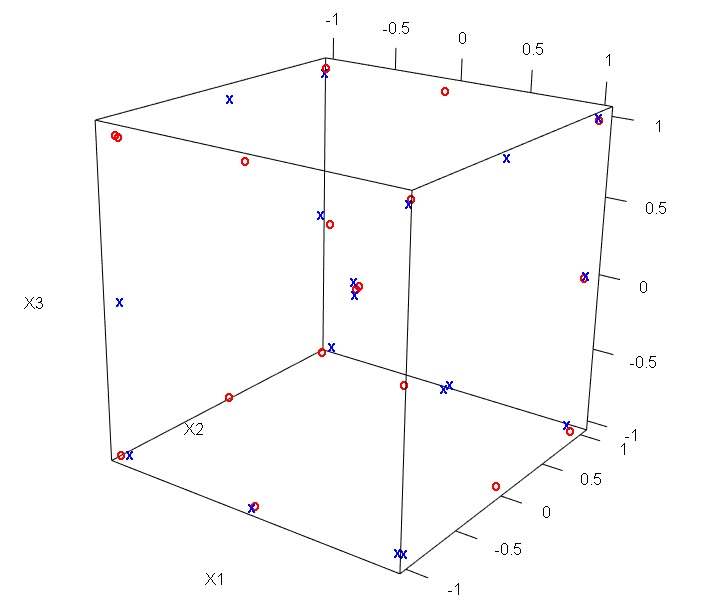
\includegraphics[scale=0.65]{CS_design.jpg}      %width=\textwidth
\caption{MSE(D)-optimal design \#$1$. Colours (blue and red) and symbols (`x' and `o') serve as block indicators. }
\label{fig::CS_design}
\end{center}
\end{figure} 

As for the time costs, on average an optimal design was found in $13-15$ hours, which was acceptable in this particular case. Sometimes, however, it took up to $20-24$ hours, so some extra time allowance should be accounted for when using these criteria and this search algorithm and/or the extensive sampling might be replaced by a less demanding alternative. 

%%% MSE(D)-optimal designs, WITH centre points: DP, LoF(DPs) and MSE(D) -- LoF as Ds for potential terms
\newpage
[OE: I'm not sure we need to include the following: looking at what would have happened if we could afford $5$ levels.]

Although the primary choice of the number of levels of each factor is $3$, the number of experimental runs would allow for $5$ levels so that all of the potential terms can be estimated. So we considered one more compound criterion which has a different lack-of-fit component: $DP_S$-- optimality for potential terms in the full (third-order polynomial) model, arising from the $D_S$-optimality that was suggested by \cite{Atkinson2007} (page $360$) in the context of model discrimination:
\begin{align}
\label{eq::crit2}
&\left[\left|\bm{\tilde{M}}\right|^{-1/p}\mathrm{F}(p,d,\alpha_{\!_{DP}})\right]^{\kappa_{\!_{DP}}} \times  \left[|\bm{\tilde{L}}|^{-1/q}F_{q,d_B;1-\alpha_{LoF}}\right]^{\kappa_{\!_{LoF}}}\times \notag\\ & \left[|\bm{\tilde{M}}|^{-1}\exp\left(\frac{1}{N}\sum_{i=1}^{N}\log(1+\bm{\tilde{\beta}}_{2i}'\bm{X}_q^{T}\bm{Q}\bm{X}_1\bm{\tilde{M}}^{-1}\bm{X}_1^{'}\bm{Q}\bm{X}_q\bm{\tilde{\beta}}_{2i})\right)\right]_{.}^{\kappa_{\!_{MSE}}/p}
\end{align}

This criterion further on will be referred to as the ``full'' criterion, and we shall explore how this would affect the resulting designs.

The summary of the corresponding optimal designs is given in Table \ref{tab::MSE(D)_caseCPLoF}: the `new' lack-of-fit component is denoted by DP*s. The notions of `No CP'  and `CP' efficiencies are the same as previously. For each design we calculated its $LoF(DP)$-value, so that we could assess how they would perform in terms of the criterion (\ref{eq::LoFDP_criterion}). The performances of the optimal designs are summarised in Table \ref{tab::MSE(D)_caseCPLoF}. In order to illustrate general tendencies in the designs' appearances, designs optimal with respect to the criterion with equal weights, for two values of $\tau^2$ are provided in Table \ref{tab::Full_designs}.

\begin{table}[h]
\centering
\caption{Case-study. Properties of ``Full'' MSE(D)-optimal blocked designs, with two centre points per block}
\label{tab::MSE(D)_caseCPLoF}
\resizebox{\textwidth}{!}}  & \multicolumn{4}{l}{\textbf{CP Efficiency,\%}}& \multicolumn{1}{l}{\textbf{Relative}}                          \\
   & \textbf{DP}       & \textbf{DP*s}    & \textbf{MSE(D)}   & \textbf{PE}        & \textbf{LoF}        & \textbf{DP} & \textbf{DP*s}  & \textbf{LoF(DP)}   & \textbf{MSE(D)}  &  \textbf{DP}  &  \textbf{DP*s} & \textbf{LoF(DP)}   & \textbf{MSE(D)} & \textbf{Efficiency,\%} \\
1 & 1/3 & 1/3 & 1/3 & \multicolumn{1}{|r}{14} & \multicolumn{1}{r|}{11} & 80.58 & 69.38 & 87.05 & 91.74 & \multicolumn{1}{|r}{84.46} & 79.90 & 94.36 & \multicolumn{1}{r|}{92.46} & 94.42 \\
2 & 0.4 & 0.2 & 0.4 & \multicolumn{1}{|r}{14} & \multicolumn{1}{r|}{11} & 83.90 & 61.18 & 85.36 & 57.47 & \multicolumn{1}{|r}{87.93} & 70.46 & 92.52 & \multicolumn{1}{r|}{57.92} & 95.83 \\
3 & 0.25 & 0.25 & 0.5 & \multicolumn{1}{|r}{13} & \multicolumn{1}{r|}{12} & 79.93 & 68.24 & 87.06 & 94.05 & \multicolumn{1}{|r}{83.77} & 78.59 & 94.37 & \multicolumn{1}{r|}{94.79} & 96.32 \\
4 & 1 & 0 & 0 & \multicolumn{1}{|r}{20} & \multicolumn{1}{r|}{5} & 95.41 & 0.00 & 62.13 & 95.24 & \multicolumn{1}{|r}{100.00} & 0.00 & 67.34 & \multicolumn{1}{r|}{95.98} & 95.41 \\
5 & 0 & 1 & 0 & \multicolumn{1}{|r}{14} & \multicolumn{1}{r|}{11} & 62.01 & 86.83 & 92.98 & 74.95 & \multicolumn{1}{|r}{64.99} & 100.00 & 100.78 & \multicolumn{1}{r|}{75.53} & 86.83 \\
6 & 0 & 0 & 1 & \multicolumn{1}{|r}{14} & \multicolumn{1}{r|}{11} & 88.31 & 0.00 & 88.35 & 99.23 & \multicolumn{1}{|r}{92.55} & 0.00 & 95.77 & \multicolumn{1}{r|}{100.00} & 99.23 \\
 & & & & & & & & & & & & & & \\
   & \multicolumn{3}{l}{\textbf{Criteria, $\bm{\tau^2=1/q}$}} & \multicolumn{2}{l}{\textbf{DoF}} & \multicolumn{4}{l}{\textbf{No CP Efficiency,\%}}  & \multicolumn{4}{l}{\textbf{CP Efficiency,\%}}& \multicolumn{1}{l}{\textbf{Relative}}                          \\
    & \textbf{DP}       & \textbf{DP*s}    & \textbf{MSE(D)}   & \textbf{PE}   & \textbf{LoF}        & \textbf{DP} & \textbf{DP*s}  & \textbf{LoF(DP)}   & \textbf{MSE(D)}  &  \textbf{DP} & \textbf{DP*s} & \textbf{LoF(DP)}   & \textbf{MSE(D)} & \textbf{Efficiency,\%} \\
1 & 1/3 & 1/3 & 1/3 & \multicolumn{1}{|r}{14} & \multicolumn{1}{r|}{11} & 80.14 & 69.01 & 87.70 & 91.41 & \multicolumn{1}{|r}{83.99} & 81.43 & 90.34 & \multicolumn{1}{r|}{92.07} & 93.97\\
2 & 0.4 & 0.2 & 0.4 & \multicolumn{1}{|r}{14} & \multicolumn{1}{r|}{11} & 83.76 & 61.29 & 88.28 & 94.41 & \multicolumn{1}{|r}{87.79} & 72.31 & 90.95 & \multicolumn{1}{r|}{95.09} & 96.04\\
3 & 0.25 & 0.25 & 0.5 & \multicolumn{1}{|r}{12} & \multicolumn{1}{r|}{13} & 79.66 & 64.43 & 84.44 & 94.84 & \multicolumn{1}{|r}{83.49} & 76.02 & 86.99 & \multicolumn{1}{r|}{95.52} & 95.20\\
4 & 1 & 0 & 0 & \multicolumn{1}{|r}{20} & \multicolumn{1}{r|}{5} & 95.41 & 0.00 & 90.63 & 95.66 & \multicolumn{1}{|r}{100.00} & 0.00 & 93.37 & \multicolumn{1}{r|}{96.35} &  95.41\\
5 & 0 & 1 & 0 & \multicolumn{1}{|r}{14} & \multicolumn{1}{r|}{11} & 59.81 & 84.75 & 86.15 & 72.05 & \multicolumn{1}{|r}{62.68} & 100.00 & 88.75 & \multicolumn{1}{r|}{72.57} & 84.75 \\
6 & 0 & 0 & 1 & \multicolumn{1}{|r}{14} & \multicolumn{1}{r|}{11} & 88.73 & 0.00 & 90.57 & 99.29 & \multicolumn{1}{|r}{92.99} & 0.00 & 93.30 & \multicolumn{1}{r|}{100.00} & 99.29
\end{tabular}
}
\end{table}

\begin{table}[h]
\centering
\caption{Case-study. Designs \#$1$ from Table \ref{tab::MSE(D)_caseCPLoF}, $\tau^2=1$ (left) and $\tau^2=1/q$ (right)}
\begin{center}
\label{tab::Full_designs}
\scalebox{0.73}{
\begin{tabular}{rrrrrrrr|r|rrrrlrrr}
-1 & -1 & 0 &  & -1 & -1 & -1 &  &  &  & -1 & -1 & -1 &  & -1 & -1 & -1 \\
-1 & -1 & 1 &  & -1 & -1 & 0 &  &  &  & -1 & -1 & 0.5 &  & -1 & -1 & 0.5 \\
-1 & 0 & -1 &  & -1 & -1 & 1 &  &  &  & -1 & -0.5 & 1 &  & -1 & -0.5 & 1 \\
-1 & 0.5 & 1 &  & -1 & 0.5 & 1 &  &  &  & -1 & 0 & -0.5 &  & -1 & 1 & -1 \\
-1 & 1 & -1 &  & -1 & 1 & -1 &  &  &  & -1 & 1 & -1 &  & -1 & 1 & 1 \\
-1 & 1 & 0.5 &  & -1 & 1 & 0.5 &  &  &  & -1 & 1 & 1 &  & -0.5 & -1 & -0.5 \\
-0.5 & 1 & 1 &  & -0.5 & -0.5 & 1 &  &  &  & -0.5 & 1 & 0 &  & -0.5 & 0.5 & -1 \\
0 & -1 & -1 &  & -0.5 & 1 & -0.5 &  &  &  & 0 & -1 & 1 &  & 0 & -1 & 1 \\
0 & 0 & 0 &  & 0 & -1 & -1 &  &  &  & 0 & 0 & 0 &  & 0 & 0 & 0 \\
0 & 0 & 0 &  & 0 & 0 & 0 &  &  &  & 0 & 0 & 0 &  & 0 & 0 & 0 \\
0.5 & -1 & 1 &  & 0 & 0 & 0 &  &  &  & 0 & 1 & 1 &  & 0 & 1 & 1 \\
0.5 & 1 & -1 &  & 0.5 & -1 & 1 &  &  &  & 0.5 & -0.5 & -1 &  & 0.5 & 1 & -0.5 \\
1 & -1 & -1 &  & 0.5 & 1 & -1 &  &  &  & 1 & -1 & -1 &  & 1 & -1 & -1 \\
1 & -1 & 0.5 &  & 1 & -1 & -1 &  &  &  & 1 & -1 & 0 &  & \textbf{1} & \textbf{-1} & \textbf{1} \\
1 & -0.5 & 1 &  & 1 & -1 & 0.5 &  &  &  & 1 & 0.5 & 1 &  & \textbf{1} & \textbf{-1} & \textbf{1} \\
1 & 0.5 & -1 &  & 1 & -0.5 & -0.5 &  &  &  & \textbf{1} & \textbf{1} & \textbf{-1} &  & 1 & 0 & -0.5 \\
1 & 1 & -0.5 &  & 1 & 0.5 & -1 &  &  &  & \textbf{1} & \textbf{1} & \textbf{-1} &  & 1 & 0.5 & 1 \\
1 & 1 & 1 &  & 1 & 1 & 1 &  &  &  & 1 & 1 & 0.5 &  & 1 & 1 & 0.5
\end{tabular}
}
\end{center}
\end{table}

In case of $\tau^2=1$ all pure error degrees of freedom (except for the $2$ coming from the replicated centre points) occur from $12$ points duplicated in different blocks; in case of $\tau^2=1/q$ (i.e. $\tau^2=0.1$) two `corner' points are replicated within the same block (they are highlighted in Table \ref{tab::Full_designs}). Quite a few experimental units would receive an `intermediate' $\pm 0.5$ dosage of at least one product, and as this did not comply with the demands of the experimenters, the choice was still made in favour of the three-level design in Table \ref{tab::CS_Design}. 